\chapter{The first appendix}

Text for the first appendix goes here.

\section{Appendix section}

Text for a section in the first appendix goes here.

\verb+test ทดสอบฟอนต์ teletype ภาษาไทย+

\texttt{test ทดสอบฟอนต์ teletype ภาษาไทย}

\chapter{\ifcpe คู่มือการใช้งานระบบ\else Manual\fi}
\section{โครงสร้างไดเรกทอรีสำหรับข้อมูลนำเข้าของโปรแกรม}
\label{apd:snd_apd}
ข้อมูลนำเข้าของโปรแกรมต้องมีการจัดเก็บตามโครงสร้างไดเรกทอรี่และมีการตั้งชื่อไฟล์ดังที่แสดงด้านล่าง

\begin{forest}
  for tree={
    font=\ttfamily,
    grow'=0,
    child anchor=west,
    parent anchor=south,
    anchor=west,
    calign=first,
    inner xsep=7pt,
    edge path={
      \noexpand\path [draw, \forestoption{edge}]
      (!u.south west) +(7.5pt,0) |- (.child anchor) pic {folder} \forestoption{edge label};
    },
    % style for your file node 
    file/.style={edge path={\noexpand\path [draw, \forestoption{edge}]
      (!u.south west) +(7.5pt,0) |- (.child anchor) \forestoption{edge label};},
      inner xsep=2pt,font=\small\ttfamily
                 },
    before typesetting nodes={
      if n=1
        {insert before={[,phantom]}}
        {}
    },
    fit=band,
    before computing xy={l=15pt},
  } 
[root-folder
  [data
    [exam-courses-faculty
        [01.in,file]
        [02.in,file]
        [03.in,file]
        [...,file]
        [19.in,file]
        [20.in,file]
        [21.in,file]
    ]
    [all-exam-courses.in,file]
    [conflicts.in,file]
    [enrolled-courses.in,file] 
    [faculty-capacity.in,file]
    [regist.in,file]
    [regist-studentid.in,file]
  ]
  [final\_exam\_graph\_coloring.py,file]
  [penalty\_calc.py,file]
  [start\_penalty\_report.py,file]
  [start\_scheduler.py,file]
  [std\_data\_to\_json.py,file]
]
\end{forest}
\begin{figure}
    \begin{center}
      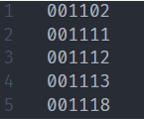
\includegraphics[]{images/all_exam1.png}
    \end{center}
    \caption[ตัวอย่างไฟล์รายวิชาที่มีสอบ]{ตัวอย่างไฟล์รายวิชาที่มีสอบ}
    \label{fig:all_courses}     
\end{figure}
\begin{figure}
    \begin{center}
    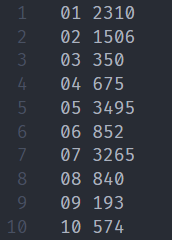
\includegraphics[]{images/capacity1.png}
    \end{center}
    \caption[ตัวอย่างไฟล์ความจุห้องสอบ]{ตัวอย่างไฟล์ความจุห้องสอบ}
    \label{fig:capacity}     
\end{figure}
\begin{figure}
    \begin{center}
      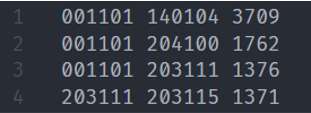
\includegraphics[]{images/conflicts1.png}
    \end{center}
    \caption[ตัวอย่างไฟล์คู่วิชาที่มีนักศึกษาลงทะเบียนพร้อมกัน]{ตัวอย่างไฟล์คู่วิชาที่มีนักศึกษาลงทะเบียนพร้อมกัน}
    \label{fig:conflicts}     
\end{figure}
\begin{figure}
    \begin{center}
      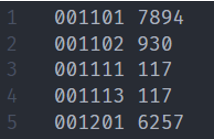
\includegraphics[]{images/courses1.png}
    \end{center}
    \caption[ตัวอย่างไฟล์วิชาที่มีนักศึกษาลงทะเบียน]{ตัวอย่างไฟล์วิชาที่มีนักศึกษาลงทะเบียน}
    \label{fig:courses}     
\end{figure}
\begin{figure}
    \begin{center}
      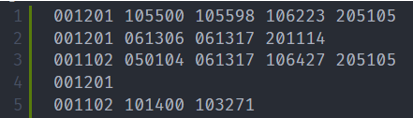
\includegraphics[]{images/regist1.png}
    \end{center}
    \caption[ตัวอย่างไฟล์ลงทะเบียนของนักศึกษา]{ตัวอย่างไฟล์ลงทะเบียนของนักศึกษา}
    \label{fig:regist}     
\end{figure}
\begin{figure}
    \begin{center}
      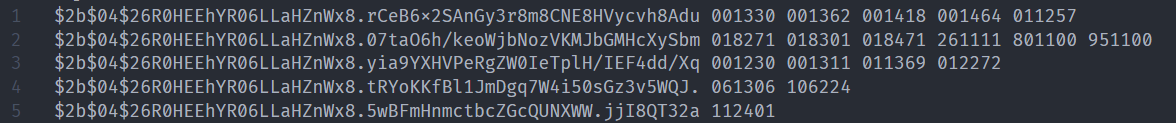
\includegraphics[width=\linewidth]{images/regist_hashed.png}
    \end{center}
    \caption[ตัวอย่างไฟล์ลงทะเบียนของนักศึกษาที่มีรหัสนักศึกษา]{ตัวอย่างไฟล์ลงทะเบียนของนักศึกษาที่มีรหัสนักศึกษา}
    \label{fig:regist_hashed}     
\end{figure}

\newcommand\str[1]{\texttt{#1}}
\CIreply{รบกวนใส่ \texttt{str} commands ให้แต่ละชื่อด้วยครับ}
\CIreply{ภาพ vs รูป}
\begin{itemize}
  \item ในโฟลเดอร์ \str{data} ประกอบไปด้วยไฟล์ all-exam-course.in, faculty-capacity.in, conflicts.in,
  enrolled-courses.in, regist.in, regist-studentid.in รวมทั้งหมดจำนวน 6 ไฟล์ แต่ละไฟล์ เป็นไฟล์ text 
  \item ในไฟล์ all-exam-course.in แต่ละบรรทัดประกอบด้วย <รหัสวิชาที่มีการจัดสอบ> หนึ่งบรรทัดต่อหนึ่งรหัสวิชา ตัวอย่างดังภาพที่~\ref{fig:all_courses}
  \item ในไฟล์ faculty-capacity.in แต่ละบรรทัดประกอบด้วย รหัสคณะและจำนวนความจุรวมของห้องสอบของคณะนั้น ๆ มีรูปแบบดังนี้ <รหัสคณะ> <ความจุห้องสอบคณะ> แต่ละส่วนคั่นด้วย เว้นวรรค (space) หนึ่งบรรทัดต่อหนึ่งคณะ ตัวอย่างดังภาพที่~\ref{fig:capacity}
  \item ในไฟล์ conflicts.in แต่ละบรรทัดประกอบด้วย รหัสวิชาสองวิชาที่มีนักศึกษาลงทะเบียนพร้อมกันในภาคการศึกษานั้น ๆ และ จำนวนนักศึกษาที่ลงทะเบียนคู่วิชานี้ มีรูปแบบดังนี้ <รหัสวิชา> <รหัสวิชา> <จำนวนนักศึกษา> แต่ละส่วนคั่นด้วย เว้นวรรค (space) ตัวอย่างดังภาพที่~\ref{fig:conflicts}
  \item ในไฟล์ enrolled-courses.in แต่ละบรรทัดประกอบด้วย รหัสวิชาและจำนวนนักศึกษาที่ลงทะเบียนในวิชานั้น ๆ มีรูปแบบดังนี้ <รหัสวิชา> <จำนวนนักศึกษา> แต่ละส่วนคั่นด้วย เว้นวรรค (space) ตัวอย่างดังภาพที่~\ref{fig:courses}
  \item ในโฟลเดอร์ data/exam-courses-faculty ประกอบไปด้วยไฟล์ 01.in ถึง 21.in ซึ่งเป็นไฟล์ text โดยตั้งชื่อไฟล์ตามรหัสคณะ ในแต่ละไฟล์ประกอบด้วย รหัสวิชาที่มีการจัดสอบ หนึ่งบรรทัดต่อหนึ่งรหัสวิชา ตัวอย่างดังภาพที่~\ref{fig:all_courses} 
  \item ในไฟล์ regist.in แต่ละบรรทัดประกอบด้วย ข้อมูลลงทะเบียนของนักศึกษาหนึ่งคน ซึ่งประกอบด้วยด้วยรหัสวิชาทั้งหมดที่นักศึกษาคนนั้นลงทะเบียน มีรูปแบบดังนี้ <รหัสวิชา> <รหัสวิชา> <รหัสวิชา> ... แต่ละวิชาคั่นด้วย เว้นวรรค (space) ตัวอย่างดังภาพที่~\ref{fig:regist}
  \item ในไฟล์ regist-studentid.in แต่ละบรรทัดประกอบด้วย ข้อมูลลงทะเบียนของนักศึกษาหนึ่งคน \\ ประกอบด้วยด้วยรหัสนักศึกษาและวิชาทั้งหมดที่นักศึกษาคนนั้นลงทะเบียน มีรูปแบบดังนี้ \\ <รหัสนักศึกษา> <รหัสวิชา> <รหัสวิชา> <รหัสวิชา> ... แต่ละส่วนคั่นด้วย เว้นวรรค (space) \\ ตัวอย่างดังภาพที่~\ref{fig:regist_hashed}
  โดยในตัวอย่างได้มีการแฮช (hash) รหัสนักศึกษา เพื่อปกป้องข้อมูลส่วนตัวของนักศึกษา
\end{itemize}

\section{การติดตั้ง Python ก่อนการใช้งานโปรแกรม}

\CIreply{ใช้ teletype font สำหรับส่วนที่เกี่ยวข้องกับ command line}
\paragraph{การติดตั้ง Python}
\begin{enumerate}
  \item ไปยัง \url{https://www.python.org/downloads/} เพื่อดาวน์โหลดตัว setup ของ Python
  \item เมื่อเปิดไฟล์ setup ให้ติ๊กถูกที่ช่อง Add python 3.x to PATH ด้วย จากนั้น install ตามปกติ
  \item เมื่อติดตั้ง Python เสร็จแล้ว ให้ทดลองตรวจสอบว่า Python นั้นติดตั้งสำเร็จ โดยการเปิด cmd หรือ powershell แล้วใช้คำสั่ง 
  \begin{verbatim}
    py --version
  \end{verbatim}
  จะแสดง version ของ Python ที่ติดตั้งลงในเครื่อง
\end{enumerate}

\paragraph{การติดตั้งแพคเกจ \str{networkx}}
\begin{enumerate}
  \item เมื่อติดตั้ง Python สำเร็จแล้ว ให้เปิด cmd หรือ powershell จากนั้นใช้คำสั่ง
  \begin{verbatim}
    pip install networkx
  \end{verbatim}
  \item หากมีการยืนยันให้กด \verb+y+ และ enter เพื่อทำการติดตั้งแพคเกจ
  \item เมื่อติดตั้งแพคเกจเรียบร้อยแล้ว ถือว่าเสร็จสิ้นการเตรียมการ สามารถเรียกใช้งานโปรแกรมจัดตารางสอบได้ทันที
\end{enumerate}

\section{วิธีการใช้งานโปรแกรม}
\begin{enumerate}
    \item จัดเตรียมไฟล์ข้อมูลนำเข้าต่าง ๆ ตามที่ได้ระบุไว้ใน \ref{apd:snd_apd} ให้เรียบร้อย
    \item เปิดไฟล์ \verb+final_exam_graph_coloring.py+
    \item ทำการแก้ไข path ของไฟล์ข้อมูลนำเข้าต่าง ๆ ให้ตรงตามที่กำหนด หากได้ตั้งชื่อไฟล์ และจัดแยกไฟล์ต่าง ๆ ไว้ตามโฟลเดอร์ที่กำหนดแล้วไม่จำเป็นต้องแก้ไขตัวแปร path ใด ๆ
    \item ทำการแก้ไขจำนวน slot ที่ใช้สอบ โดยแก้ไขที่ตัวแปร \verb+TOTAL_SLOTS+
\end{enumerate}
ในกรณีที่ต้องการจัดตารางสอบด้วยอัลกอริทึมเพียงวิธีเดียว สามารถเรียกใช้งานโปรแกรมผ่าน console หรือ terminal เช่น cmd หรือ powershell ได้ด้วยคำสั่ง 
\begin{verbatim}
    py final_exam_graph_coloring.py [OPTION]
\end{verbatim}
ซึ่ง \verb+OPTION+ เป็นไปได้ 4 แบบ ได้แก่ [-deg, -std, -deg-bfs, -std-bfs]

\begin{verbatim}
    ตัวอย่างการเรียกใช้งานโปรแกรม
    py final_exam_graph_coloring.py -deg
\end{verbatim}

\noindent ในกรณีที่ต้องการจัดตารางสอบทั้งหมด 4 วิธี สามารถเรียกใช้งานโปรแกรมผ่าน console หรือ terminal เช่น cmd หรือ powershell ได้ด้วยคำสั่ง
\begin{verbatim}
    py start_scheduler.py
\end{verbatim}
\section{วิธีการใช้งานโปรแกรมคำนวณค่า penalty}
\begin{enumerate}
    \item จัดเตรียมไฟล์ข้อมูลนำเข้าต่าง ๆ ตามที่ได้ระบุไว้ใน \ref{apd:snd_apd} ให้เรียบร้อย
    \item เปิดไฟล์ \verb+penalty_calc.py+
    \item ทำการแก้ไข path ของไฟล์ข้อมูลนำเข้าต่าง ๆ ให้ตรงตามที่กำหนด หากได้ตั้งชื่อไฟล์ และจัดแยกไฟล์ต่าง ๆ ไว้ตามโฟลเดอร์ที่กำหนดแล้วไม่จำเป็นต้องแก้ไขตัวแปร path ใด ๆ
    \item ทำการแก้ไขจำนวน slot ที่ใช้สอบให้ตรงกับ solution ของตารางสอบที่จัดโดยโปรแกรม โดยแก้ไขที่ตัวแปร \verb+TOTAL_SLOTS+
\end{enumerate}
ในกรณีที่ต้องการคิดคำนวณค่า penalty ของตารางสอบเพียง 1 solution สามารถเรียกใช้งานโปรแกรมผ่าน console หรือ terminal เช่น cmd หรือ powershell ได้ด้วยคำสั่ง 
\begin{verbatim}
    py penalty_calc.py <solution_file>
\end{verbatim}
โดยที่ \verb+<solution_file>+ คือ path ของไฟล์ solution ตารางสอบที่ได้จากโปรแกรมจัดตารางสอบ

\begin{verbatim}
    ตัวอย่างการเรียกใช้งานโปรแกรมคำนวณค่า penalty
    py penalty_calc.py solution/graph-coloring-solution-deg.txt
\end{verbatim}

\noindent ในกรณีที่ต้องการคิดคำนวณค่า penalty ของตารางสอบทั้งหมด 4 วิธี สามารถเรียกใช้งานโปรแกรมคำนวณค่า penalty ผ่าน console หรือ terminal เช่น cmd หรือ powershell ได้ด้วยคำสั่ง
\begin{verbatim}
    py start_penalty_report.py
\end{verbatim}
โดยให้เปิดไฟล์ \verb+start_penalty_report.py+ เพื่อแก้ไขตัวแปร \verb+solution_folder+ ให้ชี้ไปยังโฟลเดอร์ที่เก็บ solution ตารางสอบทั้งหมดที่เป็น output ของโปรแกรมจัดตารางสอบให้ถูกต้องก่อนการเรียกใช้งานคำสั่งด้านบน